\documentclass{cdl_sponsor}


%%%%%%%%%%%%%%%%%%%%%%%%%%%%%%%%%%%%%%%%
% Définition des variables de la classe cdl_sponsor

\DefTitre{Capitole du Libre 2015}
\DefSousTitre{Dossier de Sponsoring}
\DefAuteur{Toulibre}
\DefWeb{http://2015.capitoledulibre.org}

%%%%%%%%%%%%%%%%%%%%%%%%%%%%%%%%%%%%%%%%
% Informations du document (pour pdflatex)
\ifpdf
  \hypersetup{pdftitle={\SousTitre}}
  \hypersetup{pdfauthor={\Auteur}}
  \hypersetup{pdfsubject={\Titre}}
  \hypersetup{pdfcreator={\Auteur}}
  \hypersetup{pdfproducer={\Auteur}}
  \hypersetup{pdfkeywords={}}
\fi

\begin{document}

\thispagestyle{empty} % Remove page numbering on this page

%----------------------------------------------------------------------------------------
%	TITLE SECTION
%----------------------------------------------------------------------------------------

\colorbox{Cdl}{
	\parbox[t]{1.0\linewidth}{
		\centering \fontsize{50pt}{80pt}\selectfont % The first argument for fontsize is the font size of the text and the second is the line spacing - you may need to play with these for your particular title
		\vspace*{0.7cm} % Space between the start of the title and the top of the grey box
		
		\hfill Capitole du Libre 2015		\\
		\hfill Dossier \textit{Sponsoring}  \\
		\hfill Toulibre  					\\\par
		
		\vspace*{0.7cm} % Space between the end of the title and the bottom of the grey box
	}
}

%----------------------------------------------------------------------------------------

\vfill % Space between the title box and author information

%----------------------------------------------------------------------------------------
%	AUTHOR NAME AND INFORMATION SECTION
%----------------------------------------------------------------------------------------
{\centering \large 
\hfill Association Toulibre \\
\hfill \url{http://toulibre.org} \\
\hfill \url{http://capitoledulibre.org} \\
\hfill \url{contact@capitoledulibre.org} \\
%\HRule{1pt}} % Horizontal line, thickness changed here
}
%----------------------------------------------------------------------------------------
\clearpage

\section{Présentation des logiciels libres}

	% Partie logiciels libres
% macros personnelles 
\newcommand{\lls}{logiciels libres~}
%%%%%%%%%%%%%%%%%%%%%%%%%%%%%%%%%%%%%%%%%%%%%%%%%%%%%%%%%%%

\citation{Je peux expliquer le logiciel libre en trois mots : \\ Liberté, Égalité, Fraternité.}{Richard Matthew \bsc{Stallman}}

\subsection{Quelques points d’histoire}
\begin{minipage}{0.7\textwidth}
C’est aux États-Unis en 1984 que la notion de \textcolor{Cdl}{\textit{logiciel libre}} a été définie par \textcolor{Cdl}{Richard Matthew \bsc{Stallman}} pour la première fois. Il rédigea en parallèle la \textcolor{Cdl}{\textit{licence publique générale \bsc{Gnu}}} (la \g{GPL}) permettant d’assurer et de protéger les libertés définies par le logiciel libre. Enfin, il fonde la même année la \textcolor{Cdl}{\textit{Free Software Fondation}} afin de baser son projet sur de solides bases.
\end{minipage}
\begin{minipage}{0.3\textwidth}
\begin{center}
\image{gnu.pdf}{0.8\textwidth}\\
\textit{Logo du projet \bsc{Gnu}}
\end{center}
\end{minipage}

\begin{multicols}{2}[\subsection{La philosophie des logiciels libres}]
La philosophie des \lls est le respect des libertés des utilisateurs. En les utilisant, ils ont la liberté de les \textbf{exécuter}, les \textbf{copier}, les \textbf{distribuer}, les \textbf{modifier} et enfin de les \textbf{améliorer}.

Il ne faut toutefois pas confondre logiciel gratuit et logiciel libre. Dans le premier cas, celui-ci n’assure pas forcement les quatre libertés de l’utilisateur. Les exemples les plus parlant sont certains logiciels de Google.

\textit{A contrario}, un  logiciel libre n’est pas obligatoirement gratuit. Il existe un modèle économique viable basé sur le développement ou la vente de service sur du logiciel libre. Un bon exemple est l’entreprise Red\,Hat aux États-Unis ou encore Bluemind en France.
\end{multicols}

\citationen{Think of ‘free speech’, not ‘free beer’.}{Richard Matthew \bsc{Stallman}}

Pour qu’un logiciel soit libre, celui-ci doit respecter quatre libertés essentielles :

\begin{center}
\begin{minipage}{0.8\textwidth}
\begin{center}
\textcolor{Cdl}{\large Liberté 0} \\ \textit{La liberté d'exécuter le programme comme vous voulez, pour n'importe quel usage.} \\
\textcolor{Cdl}{\large Liberté 1} \\ \textit{La liberté d'étudier le fonctionnement du programme, et de le modifier pour qu'il effectue vos tâches informatiques comme vous le souhaitez.} \\
\textcolor{Cdl}{\large Liberté 2} \\ \textit{La liberté de redistribuer des copies, donc d'aider votre voisin.} \\
\textcolor{Cdl}{\large Liberté 3} \\ \textit{La liberté de distribuer aux autres des copies de vos versions modifiées.}
\end{center}
\end{minipage}
\end{center}

\begin{multicols}{2}
La \textcolor{Cdl}{liberté 0} est essentielle pour une utilisation universelle du logiciel. Le logiciel doit pouvoir être disponible sur toutes les plateformes, et utilisable par tous.

Pour respecter les \textcolor{Cdl}{libertés 1 à 3}, le code source, ou la \g{recette}, du logiciel doit être mis à disposition des utilisateurs. Celui-ci permet à tous de pouvoir lire, étudier, modifier et améliorer le logiciel. 

L’accès aux \textcolor{Cdl}{sources} du logiciel permet aussi un contrôle des utilisateurs sur le travail du ou des créateur. Grâce à ce principe de vérification, les erreurs ou failles de sécurité peuvent être très rapidement corrigées. Pour cette raison, les logiciels libres font références en terme de sécurité et de fiabilité.
\end{multicols}

\begin{multicols}{2}[\subsection{Les formats ouverts}]
Le format des fichier est aussi une composante essentielle au développement des logiciels libres.

Un \textcolor{Cdl}{format ouvert} assure dans un premier temps la pérennité du fichier sur le long terme, et ce indépendamment d’un éditeur de logiciel. De ce fait, il sera toujours possible de lire un format ouvert, même si le logiciel initialement prévu pour le lire n’existe plus. Les formats ouverts permettent aussi la polyvalence des logiciels compatibles. L’utilisateur n’est pas obligé d’utiliser un logiciel spécifique ou encore d’utiliser un système d’exploitation particulier.
\end{multicols}

\subsection{Quelques exemples de logiciels libres}

\begin{minipage}{0.1\textwidth}
\begin{center}
\image{firefox_logo.png}{0.6\textwidth} \\\vspace{1mm}
\image{libreoffice.pdf}{0.6\textwidth}\vspace{1mm}
\image{thunderbird_logo.png}{0.6\textwidth}\vspace{1mm}
\image{vlc.pdf}{0.6\textwidth}\vspace{1mm}
\image{gimp.pdf}{0.6\textwidth}
\end{center}
\end{minipage}
\begin{minipage}{0.75\textwidth}
\begin{multicols}{2}
Les logiciels libres sont utilisés par énormément de monde, parfois sans qu’ils en aient connaissance. 

On peut par exemple citer le navigateur Web \textcolor{Cdl}{Firefox}, le logiciel de rédaction de documents \textcolor{Cdl}{LibreOffice}, le client de courriels \textcolor{Cdl}{Thunderbird}, le lecteur multimédia \textcolor{Cdl}{VLC} ou encore le logiciel de traitement d’images \textcolor{Cdl}{The Gimp}.

Les logiciels libres sont aussi utilisés en très grande majorité sur les serveurs des entreprises très souvent basées sur des distribution \bsc{Gnu}/Linux comme \textcolor{Cdl}{Debian} ou \textcolor{Cdl}{Red\,Hat}. Les serveurs utilisent par exemple des logiciels comme \textcolor{Cdl}{Apache}, \textcolor{Cdl}{MySQL} ou encore \textcolor{Cdl}{PHP}, représentant la quasi-totalité des sites Internet.
\end{multicols}
\end{minipage}
\begin{minipage}{0.15\textwidth}
\begin{center}
\image{debian.pdf}{0.6\textwidth}\vspace{1mm}
\image{redhat.pdf}{0.6\textwidth}\vspace{1mm}
\image{apache.pdf}{0.6\textwidth}\vspace{1mm}
\image{mysql.pdf}{0.6\textwidth}\vspace{1mm}
\image{php.pdf}{0.6\textwidth}
\end{center}
\end{minipage}
\vspace*{\baselineskip}
\begin{multicols}{2}[\subsection{Le libre au-delà du logiciel}]
La philosophie du logiciel libre restée inchangée depuis sa création s’est cependant beaucoup développée et s’est adaptée à d’autres médias ou activité. On dénombre désormais plusieurs autres domaines basée sur le même principe :
\begin{itemize}[label=$\bullet$]
\item la \textcolor{Cdl}{culture libre} : des écrivains, des musiciens ou encore des photographes partageant sous licence libre leur travail ;
\item le \textcolor{Cdl}{matériel libre} : suite au développement récent des imprimantes 3D, de nombreuses personnes distribuent sous licence libre des objets 3D. Certaines imprimantes sont elles-même développées par des communautés et mises à disposition sous licence libre.
\item des \textcolor{Cdl}{projets libres} : les plus connus sont l’encyclopédie libre Wikipédia ou encore le site de cartographie, \mbox{OpenStreetMap}.
\end{itemize}
\end{multicols}



\section{Toulibre}

	% Partie Toulibre

\textbf{Toulibre} est une association d'utilisateurs et de développeurs de logiciels libres de la région toulousaine. Elle organise des actions visant à promouvoir, développer et démocratiser les logiciels libres dans la région Midi-Pyrénées. L'association est également concernée par la promotion des œuvres diffusées sous licences libres, et se place dans une perspective d'éducation populaire. Enfin, Toulibre se veut également être un support pour les communautés locales du libre.

\Separateur

Toulibre organise des évènements ouverts à tous :
\begin{itemize}[label=$\bullet$]
\item des rencontres régulières permettant la découverte des logiciels libres, l'aide à l'utilisation et l'installation ainsi que de leur présentation ;
\item des ateliers mensuels, permettant le développement et/ou la 
pratique régulière de certains logiciels ou technologies ;
\item des manifestations ponctuelles, dont la plus importante en termes 
de public et de portée est le \textbf{Capitole du Libre}.
\end{itemize}

L'association intervient également lors d'évènements ou dans des \textbf{espaces publics numériques} (EPN) pour proposer des ateliers sur des logiciels libres ou de l'aide pour les utiliser et les installer, par exemple :
\begin{itemize}[label=$\bullet$]
\item au \textbf{Forum numérique des seniors} en 2013 et 2014 ;
\item dans les médiathèques de Tournefeuille, Blagnac et Colomiers ;
\item au cinéma Utopia de Tournefeuille.
\end{itemize}


\section{Le Capitole du Libre}

	% Partie le Capitole du Libre

Le \href{http://capitoledulibre.org}{Capitole du Libre} est un
 évènement tout public de promotion des logiciels libres,
 organisé par l’association \href{http://toulibre.org/}{Toulibre}.
 Il se déroule à Toulouse, chaque année depuis 2009, sur un 
 weekend du mois de novembre.

Grâce à une programmation variée et de qualité, 
 le \textbf{Capitole du Libre} est aujourd’hui une référence
 parmi les manifestations consacrées aux logiciels libres. Le
 public et les orateurs y viennent plus nombreux — et
 de plusieurs pays voisins — chaque année.

Tout au long du weekend, des
 \href{http://2014.capitoledulibre.org/programme/conferences/list/}{conférences}
 et des \href{http://2014.capitoledulibre.org/programme/ateliers/list/}{ateliers pratiques}
 sur des sujets variés, aussi bien techniques que grand public, se déroulent en parallèle.


%%% \textit{freetux} : Grosses redites dans ces trois premiers paragraphes. À reformuler.

 
\Separateur

Le \textbf{Capitole du Libre} est également l'occasion de réunir des 
communautés du libre pour des conférences, \textit{lightning talks}, 
\textit{coding sprints}\dots ~ Le \textbf{Capitole du Libre} a 
accueilli plusieurs évènements depuis 2011 tels que :
\begin{itemize}[label=$\bullet$]
\item \textbf{DrupalCamp} en 2011 ;
\item \textbf{DjangoCon} en 2012 ;
\item \textbf{FranceJS} en 2013 ;
\item \textbf{LuaWorkshop} en 2013 ;
\item \textbf{OpenStack} en 2013 ;
\item \textbf{Hackfest LibreOffice}  en 2014 ;
\item \textbf{Akademy-FR} depuis la première édition !
\end{itemize}

\Separateur

Un village associatif permet également de présenter les projets des associations du libre : \href{http://liberte0.org/wiki/index.php?title=Accueil}{Liberté0},
 \href{http://wikimedia.fr/}{Wikimédia France},
 \href{http://openstreetmap.fr/}{OpenStreetMap France},
 \href{http://framasoft.net/}{Framasoft}
 ou encore \href{http://tetaneutral.net/}{Tetaneutral.net}.

\begin{center}
\image{cdl-amphi-cc-by-guillaume-paumier.jpg}{1\textwidth}
\textit{Amphithéâtre comble pour Stéphane \bsc{Bortzmayer} de l'AFNIC}
\end{center}

\subsection{Quelques chiffres}

\begin{minipage}{0.6\textwidth}
En 2014, le Capitole du Libre c'était :
\begin{itemize}[label=$\bullet$]
\item \textbf{plus de \num{1000} visiteurs} ;
\item \textbf{63~conférences} ;
\item \textbf{50~heures de conférences} filmées et disponibles en ligne ;
\item \textbf{9~flux de conférences en parallèle} tout le weekend ;
\item \textbf{21~ateliers} ;
\item \textbf{22~associations} représentées dans le village associatif ;
\item \textbf{\SI{2}{\tera o} de vidéos} sous licence libre une fois traitées.
\end{itemize}
\end{minipage}
\begin{minipage}{0.4\textwidth}
\begin{center}
\image{hall-1-photo-n7.jpg}{1\textwidth}
\end{center}
\end{minipage}

\Separateur

L’évènement est basé uniquement sur le bénévolat.
 Durant les mois de préparation et pendant tout le weekend,
 plus de \textbf{60~bénévoles} des associations et des clubs techniques
 de l’INP-ENSEEIHT se sont mobilisés pour l’élaboration du programme,
 l’accueil du public, la captation des conférences ou encore l’aide
 à l’installation des logiciels libres.


\subsection{L'édition 2015}

Comme tous les ans, nous couvrirons des thématiques à la fois techniques et grand 
public :

\begin{itemize}[label=$\bullet$]
\item \textbf{DevOps} : inaugurée en 2014, sera renouvelée et abordera Docker, le \textit{cloud} libre ;
\item \textbf{Internet Of Things \& Do It Yourself} : (re)découverte des Arduino, Raspberry Pi, objets connectés ;
\item l’\textbf{Internet libre} : autohébergement, sécurité et vie privée sur l’Internet ;
\item \textbf{Technologies Web} : NodeJS, ReactJS, AngularJS, le Web change tous les jours ;
\item \textbf{Animation 2D \& 3D} : Blender, Krita, Gimp, Inkscape, Synfig, la réalisation d'œuvres artistiques avec des outils libres ;

\item \textbf{AkademyFR} : le rendez-vous de la communauté francophone de KDE et de Qt ;
\item et nos grands classiques : culture libre et multimédia, etc.
\end{itemize}

\subsection{Un évènement accessible}

\begin{minipage}{0.4\textwidth}
\begin{center}
\image{clavier-braille-photo-jeanZ.jpg}{0.8\textwidth}
\end{center}
\end{minipage}
\begin{minipage}{0.6\textwidth}
L'accessibilité de notre évènement est un aspect que nous souhaitons
 développer afin d'inclure tous les publics, et nous veillons à ce que
 tous les ateliers et conférences soient accessibles pour les personnes
 à mobilité réduite.

2014 a été l'occasion de proposer aux visiteurs des programmes
 imprimés en braille, ce qui a permis à plusieurs déficients visuels
 de profiter pleinement de l'évènement. Dans la continuité, en 2015
 nous souhaitons proposer la traduction de certaines conférences en
 langue des signes.
\end{minipage}

\subsection{Des intervenants de qualité}

Chaque année, de nombreuses personnalités participent au Capitole du Libre. Parmi elles, on peut compter :

\begin{itemize}[label=$\bullet$]
\item Benjamin \bsc{Bayart} de \textbf{FDN}, Adrienne \bsc{Charmet} et Jérémie \bsc{Zimmermann} de \textbf{La Quadrature du Net} qui ont assuré à plusieurs reprises les conférences de clôture ;
\item Stéphane \bsc{Bortzmeyer} de l'\textbf{AFNIC} qui a présenté les dessous de l'Internet mondial ;
\item Sandrine \bsc{Mathon} de \textbf{Toulouse Métropole} qui présente chaque année les avancées de notre métropole en termes d'\textit{open data}\dots
\end{itemize} 

\subsection{Des ateliers et animations pour expérimenter}

\begin{minipage}{0.6\textwidth}

Comme rien ne vaut l'expérimentation, des animations et ateliers ludiques sont proposés tout au long du weekend. Le public est invité à venir découvrir l’impression 3D, l’autohébergement de site Web, la contribution à OpenStreetMap ou encore la programmation de son propre jeu vidéo.

\end{minipage}
\begin{minipage}{0.4\textwidth}
\begin{center}
\image{CDL2014-2953-imprimante3D-photo-jeanZ.JPG}{0.7\textwidth}
\end{center}
\end{minipage}



\section{Devenir \textit{Sponsor}}

	% Partie devenir sponsor

Capitole du Libre recherche des partenaires financer l'événement et que l'évenment reste libre et accessible au plus grand nombre de personnes. Nous proposons à tout type d'entreprises de nous aider avec différents niveaux de sponsorins détaillés ci-dessous.

\Separateur

Nous sponsoriser, c'est vous associer à cette manifestation et contribuer au Logiciel Libre. Capitole du Libre est un lieu idéal pour venir découvrir de nouveaux horizons, récolter de nouvelles idées, découvrir de nouveaux talents

	\subsection{Niveaux de sponsoring}

    \begin{center}
    \begin{tabular}{|r|c|c|c|c|c|}
        \hline  & Bronze & Argent & Or & Platine & Diamant \\
        \hline Contribution & \SI{250}{\euro} & \SI{600}{\euro} & \SI{1000}{\euro} & \SI{2000}{\euro} & \SI{3000}{\euro} \\
        \hline Limite & - & - & - & 4 & 2 \\
        \hline Logo sur l'affiche et le site web & \ding{'064} & \ding{'064} & \ding{'064} & \ding{'064} & \ding{'064}  \\
        \hline Badges sponsors & \ding{'064} & \ding{'064} & \ding{'064} & \ding{'064} & \ding{'064} \\
        \hline Dépôt d'offre d'emploi et de stage & \ding{'064} & \ding{'064} & \ding{'064} & \ding{'064} & \ding{'064} \\
        \hline Logo diffusé entre les conférences & & \ding{'064} & \ding{'064} & \ding{'064} & \ding{'064} \\
        \hline Logo au début de chaque vidéo & & & \ding{'064} & \ding{'064} & \ding{'064} \\
        \hline Logo sur les \textit{flyers} de l'événement & & & \ding{'064} & \ding{'064} & \ding{'064} \\
        \hline Texte sur le programme distribué & & & 1/4 page & 1/2 page & 1 page \\
        \hline Stand à proximité des buvettes & & & & 1 table & 2 tables \\
        \hline Remerciements lors de la conférence de clôture & & & & \ding{'064} & \ding{'064}  \\
        \hline Une idée ? Contactez-nous ! & & & & & \ding{'064} \\
        \hline Mise à disposition d'une salle privative & & & & & \ding{'064} \\
        \hline 
    \end{tabular}
    \end{center}

Note: sur les différents supports, la taille de votre logo sera proportionnelle à votre niveau de support.

	\subsection{Retour d’expérience des précédents \textit{sponsors}}
	\subsection{Budget de l’événement}

Le budget total de l'édition 2014 de Capitole du Libre s'élevait à 12000€. Les différents postes de dépense sont indiqués dans le graphique ci-dessous:

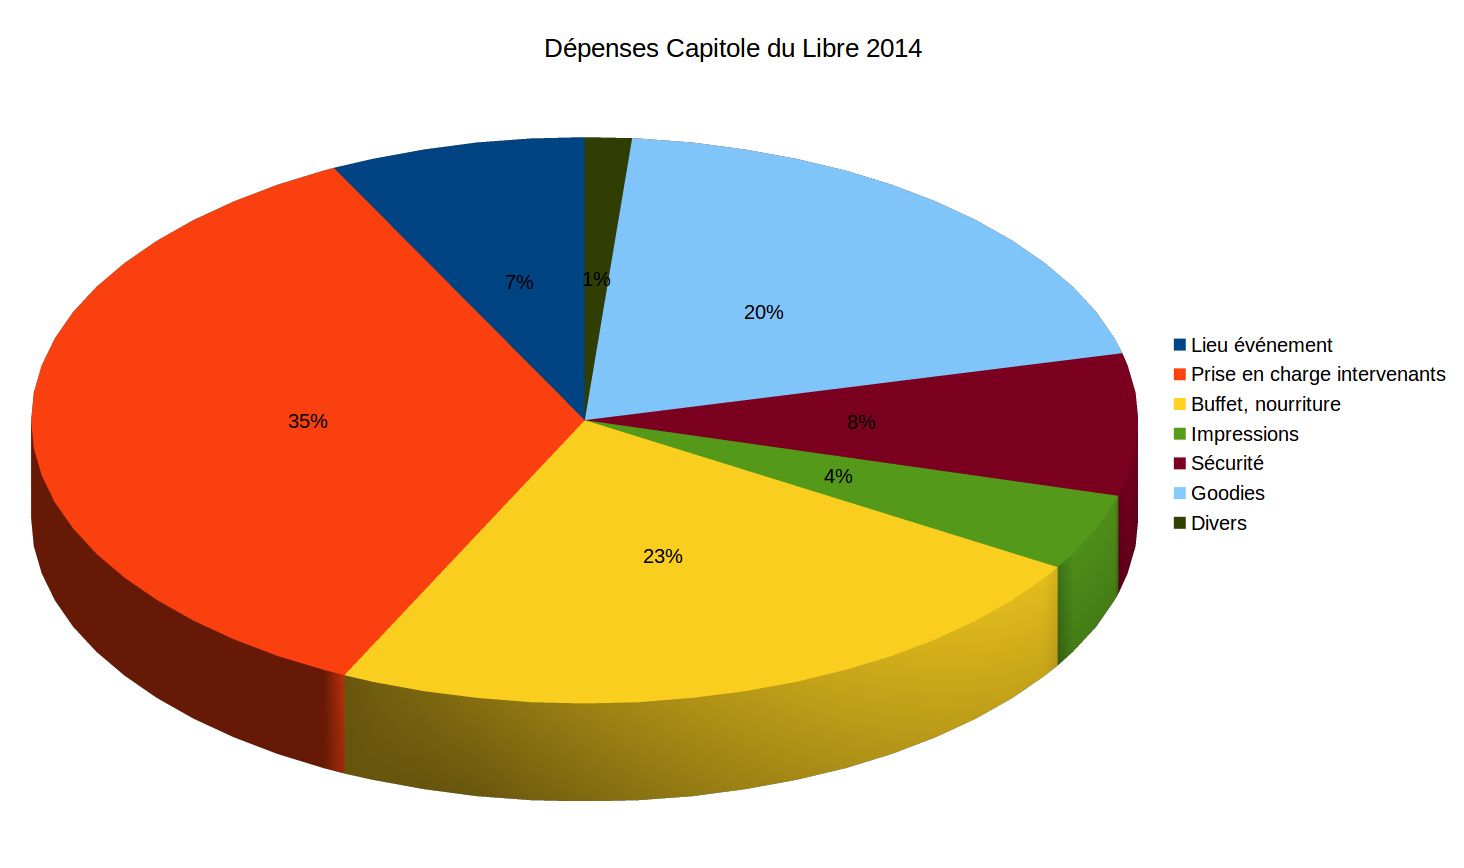
\includegraphics[scale=0.6]{Images/budget_2014.png}\\

Pour l'édition 2015 de Capitole du Libre, nous prévoyons une augmentation de notre budget à 18000 € afin principalement:
\begin{itemize}[label=$\bullet$]
\item de permettre de faire venir plus d'orateurs de plus loin afin de continuer à améliorer la qualité et la variété de nos orateurs
\item de réaliser un buffet correct le samedi soir (l'année dernière nous avions été vraiment trop juste en quantité). Ce buffet ouvert à tous et à participation libre étant un lieu d'échange privilégié lors de ce week-ends où se retrouvent orateur et particiapants des différentes thématiques.
\end{itemize}

\Separateur

Le détail des dépenses de Capitole du Libre 2015 est détaillé dans le tableau ci-dessous:

    \begin{tabular}{|l|c|}
        \hline Dépense & Montant \\
        \hline \textbf{Défraiements intervenants} & \textbf{5000 €} \\
        \hline Déplacements intervenants & 3500 € \\
        \hline Hébergement intervenants & 1500 € \\
        \hline \textbf{Hébergement manifestation} & \textbf{3000 €}\\
        \hline Chauffage & 1500 € \\
        \hline Sécurité & 1500 € \\
        \hline \textbf{Apéritif \& Repas} & \textbf{6000 € }\\
        \hline Participation repas intervenants et bénévoles & 1500 € \\
        \hline Buffet samedi soir & 4500 € \\
        \hline \textbf{Buvette} & \textbf{600€ }\\
        \hline Viénoiseries bénévoles & 150 € \\
        \hline Approvisionnement buvette & 400 € \\
        \hline Location machines à café & 50 € \\
        \hline \textbf{Goodies} & \textbf{2800 € }\\
        \hline T-Shirt Capitole du Libre 2015 & 1400 € \\
        \hline Goodies autres & 1400 € \\
        \hline \textbf{Communication} & \textbf{800 €} \\
        \hline Impression Flyyers & 100 € \\
        \hline Impression Affiches & 100 € \\
        \hline Impression Programmes & 500 € \\
        \hline Fléchage / Indications & 100 € \\
        \hline TOTAL & 18200 € \\
        \hline
    \end{tabular}

\Separateur

Les recettes 2015 sont détaillées dans le tableau ci-dessous:

    \begin{tabular}{|c|c|c|c|c|c|}
        \hline Dépense & Montant \\
        \hline Sponsors & 15 900 € \\
        \hline Dons & 300 € \\
        \hline Ventes buvette & 600 € \\
        \hline Recette boutique & 1600 € \\
        \hline TOTAL & 18200 € \\
        \hline
    \end{tabular}



\section{La ville rose}

	% Partie la ville rose

Le Capitole du Libre se déroule tous les ans à Toulouse dans l'école
 d'ingénieurs de l'ENSEEIHT (École Nationale Supérieure
 et des Télécommunications de Toulouse). 

\subsection{L'ENSEEIHT}

L'une des écoles de l'Institut Polytechnique de Toulouse, l'ENSEEIHT
 est située au centre-ville, à 10 minutes de la place du Capitole.

Sa capacité d'accueil permet de proposer plusieurs conférences et
 ateliers en parallèle, et d'accueillir jusqu'à 400 personnes dans
 l'amphithéâtre le plus grand.

\subsection{Toulouse}

La ville de Toulouse est pionnière en matière de logiciels libres,
 puisqu'elle vient de réussir sa migration à LibreOffice, la suite
 bureautique libre. Par ailleurs, Toulouse Métropole est présidente de
 \textbf{Open Data France}, l'association des collectivités
 engagées dans le mouvement \textit{open data}.


	
\section{Contact}

	% Partie contact


Pour toutes questions relatives au sponsoring du Capitole du Libre :
\begin{itemize}
\item[\logo] écrivez à \href{mailto:contact@capitoledulibre.org}{\nolinkurl{contact@capitoledulibre.org}}
\end{itemize}
\paragraph{Contact presse :}
\begin{itemize}
\item[\logo] écrivez à \href{mailto:comm@capitoledulibre.org}{\nolinkurl{comm@capitoledulibre.org}}
\end{itemize}


\section{Sources \& références}

	% Partie sources & références

\vfill
\begin{center}
\textcolor{Cdl}{Crédits images} \par
{\tiny
\textbf{Photo Capitole} : \href{https://www.flickr.com/photos/blieusong/6986608500/in/set-72157629942158013}{Benh \bsc{Lieu Song} -- CC-BY-SA~3.0} via Flickr $\bullet$ \textbf{Photo conférence \bsc{Bortzmayer}} : Guillaume Paumier CC--BY~2.0 $\bullet$ \textbf{Photo hall N7} : ?? $\bullet$ \textbf{Photo clavier braille} : ?? $\bullet$ \textbf{Photo imprimante 3D} : ?? $\bullet$ \textbf{Logo \bsc{Gnu}} : \href{https://commons.wikimedia.org/wiki/File\%3AOfficial_gnu.svg"><img width="512" alt="Official gnu" src="//upload.wikimedia.org/wikipedia/commons/thumb/3/39/Official_gnu.svg/512px-Official_gnu.svg.png}{“\bsc{Gnu} Project logo”} de \href{mailto:vcopovi@wanadoo.fr}{Victor Siame} via Wikimedia Commons $\bullet$ \textbf{Logo Audacity} : \href{https://commons.wikimedia.org/wiki/File:Audacity_Logo.svg#/media/File:Audacity_Logo.svg}{“Audacity logo”} by Aaron Spike -- Part of Audacity source code released under GPLv2.. Licensed under GPL via Wikimedia Commons $\bullet$ \textbf{Logo Thunderbird} : ?? $\bullet$ Logo The~Gimp : \href{https://commons.wikimedia.org/wiki/File:The_GIMP_icon_-_gnome.svg#/media/File:The_GIMP_icon_-_gnome.svg}{“The GIMP icon -- Gnome”} by The GIMP's art/developer team -- The GIMP package. Licensed under GPL via Wikimedia Commons $\bullet$ \textbf{Logo LibreOffice} : ?? $\bullet$ \textbf{Logo VLC} : \href{https://commons.wikimedia.org/wiki/File:VLC_Icon.svg#/media/File:VLC_Icon.svg}{“VLC Icon”} by Richard C. G. \bsc{Øiestad} -- \url{http://www.videolan.org} $\bullet$ \textbf{Logo Firefox} : ??
%Licensed under GPL via Wikimedia Commons


}
\end{center}



\end{document}


%%%%%%%%% OLD DOSSIER SPONSORING CDL 2014 %%%%%%%%%%%%%%%%%%%%%%%%%%%%%%%%%

%\CreerTitre{Images/titre2.jpg}{Benh \bsc{Lieu Song} -- CC-BY-SA 3.0}

%\begin{Introduction}

%L'association \textbf{Toulibre} organise le \textcolor{Cdl}{15 et 16 novembre 2014} la quatrième édition du \textbf{\g{Capitole du Libre}}, un événement consacré aux Logiciels Libres, orienté à la fois vers le grand public et le public spécialisé.
%
%\Separateur
%
%Des cycles de conférences grand public, techniques et multimédia ont lieu le samedi. Le dimanche est consacré à des ateliers pratiques.
%
%\Separateur
%
%Une \textbf{\textit{Install Party}} permet à tous de découvrir et d'installer un système Libre sur son ordinateur. Des stands de démo et d'animations sont proposés au public toute la journée du samedi. Un \textbf{\g{village du libre}} permet aux associations autour du libre de présenter leur activité.
%
%\Separateur
%
%Le \textbf{Capitole du Libre} est également l'occasion de réunir des communautés du Libre pour des conférences, \textit{lightning talks}, \textit{coding sprints}\dots ~ Le \textbf{Capitole du Libre} a accueilli plusieurs conférences depuis 2011 telles que \textbf{DrupalCamp}, \textbf{DjangoCon},  \textbf{FranceJS}, \textbf{LuaWorkshop}, \textbf{OpenStack} et \textbf{Akademy-FR}.
%
%\Separateur
%
%Vous trouverez plus d'informations sur le site internet : \url{\Web}.
%\end{Introduction}
%
%\section{Conférences, démonstrations et ateliers du Capitole du Libre}
%
%Pendant tout un weekend, le Capitole du Libre propose conférences, animations et ateliers autour du Logiciel Libre et du bien commun, et accueille des événements de la communauté du Libre.
%
%\subsection{Conférences et ateliers}
%
%Les conférences et les ateliers qui seront programmés pourront aborder les thèmes suivants :
%\begin{itemize}
%\item[\logo] un cycle de \textbf{conférences grand public} couvrant des sujets comme les enjeux des Logiciels Libres, le Libre au-delà du Logiciel, Wikipédia, les aspects économiques ou sociaux du Logiciel Libre\dots ~ ;
%\item[\logo] un thème \textbf{bureautique et multimédia}, couvrant des sujets tels que la retouche d'image, la modélisation 3D, la musique assistée par ordinateur, la bureautique\dots ~ ;
%\item[\logo] un thème \textbf{technique} couvrant des sujets de développement logiciels, d'embarqué, d'administration système ou réseau\dots ~ ;
%\item[\logo] un thème \textbf{Internet Libre} couvrant les solutions qui permettent de maîtriser ses données personnelles sur la Toile ;
%\item[\logo] un thème \textbf{Arduino} et \textbf{Open Hardware} sur les aspects matériel et montages électroniques libres ;
%\item[\logo] un thème \textbf{DevOps} sur les problématiques d'automatisation du déploiement d'applications.
%\end{itemize}
%
%\Separateur
%
%Dans chaque thème, les conférences proposées seront de 20 minutes à une heure, et permettent de parler de plus de sujets dans une durée adaptée.
%
%\Separateur
%
%Depuis l'édition de 2011, les conférences ont lieu le samedi, et le dimanche est consacré aux ateliers pratiques, aussi bien pour le grand public que pour un public averti. Les thèmes pourront évoluer en fonction des propositions reçues.
%
%\Separateur
%
%Les années précédentes sont notamment intervenus Nicolas \bsc{Barcet} de \textbf{eNovance \& RedHat}, Benjamin \bsc{Bayart} de \textbf{FDN}, Stéphane \bsc{Bortzmeyer} de l'\textbf{AFNIC}, Adrienne \bsc{Charmet Alix} de \textbf{Wikimedia France}, Alix \bsc{Cazenave} et Frédéric \bsc{Couchet} de l'\textbf{April}, Claire \bsc{Gallon} de \textbf{LiberTIC}, Alexis \bsc{Kauffmann} et Pierre-Yves \bsc{Gosset} de \textbf{Framasoft}, Sandrine \bsc{Mathon} de \textbf{Toulouse Métropole}, Lucas \bsc{Nussbaum} et Stefano \bsc{Zacchiroli} de \textbf{Debian}, François \bsc{Pelligrini}, Paul \bsc{Rouget} de la \textbf{Mozilla Fondation}, Christophe \bsc{Sauthier} d'\textbf{Ubuntu-fr}, Jérémie \bsc{Zimmermann} de \textbf{La Quadrature du Net}\dots
%
%\subsection{Espace de stands et d'échanges}
%
%Lieu de passage du public, le grand hall de l'\bsc{Enseeiht} est un espace dédié aux stands pour les organisations, associations ou entreprises.
%
%\Separateur
%
%Il est possible également de poser du matériel de communication tel que \g{kakemono}, présentoirs\dots
%
%\Separateur
%
%En plus des stands, un espace convivial sera aménagé afin de permettre rencontres et discussions.
%
%\newpage
%\subsection{Install Party, Lan Party et espace démonstrations}
%
%L'\textit{install party} est un événement de promotion et de démocratisation des Logiciels Libres auprès du grand public, et un événement de rencontre des acteurs de la communauté du Logiciel Libre.
%
%\Separateur
%
%Organisé chaque année depuis 2008, il est intégré dans le Capitole du Libre depuis 2011.
%
%\Separateur
% 
%Cet événement propose :
%\begin{itemize}
%\item[\logo] un espace de démonstration de Logiciels Libres, où les visiteurs pourront poser leurs questions ou participer à des mini-ateliers ;
%\item[\logo] Des mini-présentations des différentes distributions Libres proposées (Ubuntu, Fedora, OpenSuse, LinuxMint\dots) ;
%\item[\logo] une \textit{install party}, permettant au grand public de trouver de l'aide pour installer des logiciels et distributions Libres sur leur propre ordinateur.
%\end{itemize}
%
%\subsection{Nouveautés de cette édition}
%
%Grande nouveauté du Capitole du Libre 2014 : un \textcolor{Cdl}{village associatif} va être organisé permettant ainsi de présenter de nombreuses distributions \bsc{Gnu}/Linux. Plusieurs groupes d'utilisateurs du libre seront aussi au rendez-vous pour présenter au public les dernières nouveautés technologiques libres du moment.
%
%\section{Événements hébergés}
%
%\subsection{Akademy-fr}
%
%\ImageDroitebis{Images/klogo-official-lineart_simple-128x128.png}
%%
%Akademy-fr est la déclinaison française de la conférence KDE annuelle. KDE est une communauté internationale produisant un ensemble d'applications multi-plateformes et notamment un environnement de bureau nommé Plasma Desktop.
%
%\Separateur
%
%Le but de l'Akademy-fr est d'améliorer la promotion de KDE au niveau de la France, à l'aide de conférences en français et d'ateliers orientés contribution.
%
%\subsection{Hackfest LibreOffice}
%
%\ImageDroite{Images/LO.png}
%
%LibreOffice est une suite bureautique libre et gratuite ; son interface claire et ses puissants outils vous permettent de libérer votre créativité et de développer votre productivité.
%
%\Separateur
%
%LibreOffice intègre plusieurs applications qui en font la plus puissante suite bureautique Libre et Open Source du marché. Le développement est ouvert à de nouveaux talents et de nouvelles idées, et le logiciel est testé et utilisé quotidiennement par une importante communauté d'utilisateurs dévoués.
%
%\Separateur
%
%Dans un \textit{Hackfest} les contributeurs LibreOffice se réunissent afin de coordonner dans un temps donné et dans une atmosphère détendue, le développement du produit et faire avancer le projet. Au sein de LibreOffice, cela passe par une communauté internationale de développeurs, designers, traducteurs et \g{QA triagers}.
%
%\Separateur 
%
%C'est une occasion idéale pour commencer ou continuer à participer à l'un des plus grands projets Open Source dans l'action !
%
%\section{Conditions de sponsoring}
%
%\textbf{Toulibre} offre la possibilité à des entreprises d'associer leur nom à l'événement \g{Capitole du Libre} qui touchera à la fois le grand public et le public spécialisé en informatique. Auprès du grand public, l'image des sponsors sera associée à un événement s'intéressant aux enjeux éthiques et sociaux du numérique. Auprès du public spécialisé, les sponsors se feront connaître comme acteurs du monde du Logiciel Libre.\par 
%Vous pouvez participer à l'événement financièrement ou bien en prenant en charge un poste de dépense (comme l'impression des affiches, le repas du dimanche\dots).
%
%\Separateur
%
%Selon que l'entreprise qui sponsorise est un grand compte ou une PME, le niveau des montants est différent (que se soit en service ou en monétaire).
%
%\Separateur
%
%En échange du sponsoring du Capitole du Libre par les entreprises associées à l'événement, Toulibre s'engage à :
%
%\begin{center}
%\arrayrulecolor{Cdl} 
%\begin{tabular}{|p{10cm}ccc|}
%\hline
%\rowcolor{Cdl} & \textbf{Bronze} & \textbf{Argent} & \textbf{Or} \\
%\hline\hline
%{\hfill\textit{Grand compte}} & \SI{300}{\euro} & \SI{700}{\euro} & \SI{1500}{\euro} \\ 
%
%{\hfill\textit{PME}} & \SI{200}{\euro} & \SI{500}{\euro} & \SI{900}{\euro} \\ 
%\hline\hline
%Logo sur l'affiche de l'événement\textcolor{Cdl}{*} & \textcolor{Cdl}{\ding{'064}} & \textcolor{Cdl}{\ding{'064}} & \textcolor{Cdl}{\ding{'064}} \\ 
%
%Logo sur le site internet dédié à l'événement\textcolor{Cdl}{*} & \textcolor{Cdl}{\ding{'064}} & \textcolor{Cdl}{\ding{'064}} & \textcolor{Cdl}{\ding{'064}} \\ 
%
%Logo au début de chaque vidéo\textcolor{Cdl}{*} & \textcolor{Cdl}{\ding{'064}} & \textcolor{Cdl}{\ding{'064}} & \textcolor{Cdl}{\ding{'064}} \\ 
%
%Badges sponsors & \textcolor{Cdl}{\ding{'064}} & \textcolor{Cdl}{\ding{'064}} & \textcolor{Cdl}{\ding{'064}} \\ 
%
%Remerciements lors de la conférence de clôture de l'événement & \textcolor{Cdl}{\ding{'064}} & \textcolor{Cdl}{\ding{'064}} & \textcolor{Cdl}{\ding{'064}} \\ 
%
%Logo sur le programme papier distribué aux participants\textcolor{Cdl}{*} &  & \textcolor{Cdl}{\ding{'064}} & \textcolor{Cdl}{\ding{'064}} \\ 
%
%Logo sur les flyers de l'événement\textcolor{Cdl}{*} &  & \textcolor{Cdl}{\ding{'064}} & \textcolor{Cdl}{\ding{'064}} \\ 
%
%
%Texte de description sur le programme papier distribué\textcolor{Cdl}{**} &  & \textcolor{Cdl}{\textbf{120}} & \textcolor{Cdl}{\textbf{380}} \\
%
%Espace pour un stand &  &  & \textcolor{Cdl}{\ding{'064}} \\ 
%
%Interview sur le site du Capitole du Libre &  &  & \textcolor{Cdl}{\ding{'064}} \\
%\hline
%\multicolumn{4}{r}{\textcolor{Cdl}{*} \textit{logo de taille différente : or plus grand que argent plus grand que bronze}}\\
%\multicolumn{4}{r}{\textcolor{Cdl}{**} \textit{en nombre de caractères}}\\
%
%\end{tabular}
%\end{center}
%
%\subsection{Les dépenses}
%
%Comme les années passées, les conférenciers pour les présentations et les ateliers seront défrayés. Votre participation permet également de financer le chauffage des locaux de l'\bsc{Enseeiht} que nous occupons tout le weekend, ainsi qu'un poste de secours obligatoire pour un événement de cette ampleur. L'apéritif dînatoire du samedi soir est en partie financé par la participation libre des convives. Tout le public y est invité.
%
%\Separateur
%
%Le Capitole du Libre est organisé exclusivement par les \textbf{bénévoles} de l'association \textbf{Toulibre} et des \textbf{clubs info, vidéo et animation de l'\bsc{ENSEEIHT}}.
%
%\Separateur
%Le budget du Capitole du Libre s'élève à environ \SI{10000}{\euro}.
%
%\newpage
%\subsection{Ils nous ont soutenu en 2013}
%
%\begin{center}
%{\Large \textcolor{Cdl}{Partenaires Or}}
%
%\urllogoau{http://www.enovance.com}{enovance.png}\hspace{1cm}
%\urllogoau{www.kdab.com}{kdab.png}\hspace{1cm}
%\urllogoau{http://www.logilab.fr}{logilab.png} \\
%\urllogoau{http://makina-corpus.com}{makina-corpus.png}\hspace{1cm}
%\urllogoau{http://boards.openpandora.org/page/homepage.html}{openpandora.png}\hspace{1cm}
%\urllogoau{http://www.sierrawireless.com}{sierra-wireless.png}
%
%\Separateur
%
%{\Large \textcolor{Cdl}{Partenaires Argent}}
%
%\Separateur
%
%\urllogoag{http://www.objectif-libre.com}{objectif-libre.png}
%
%\Separateur
%
%{\Large \textcolor{Cdl}{Partenaires Bronze}}
%
%\Separateur
%
%\urllogobr{http://blue-mind.net}{bluemind.jpg} \hspace{1cm}
%\urllogobr{http://free-electrons.com}{free-electrons.png}\hspace{1cm}
%\urllogobr{http://www.nfrance.com}{nfrance-conseil.png} \\
%\urllogobr{http://osones.com}{osones.png} \hspace{1cm}
%\urllogobr{http://www.solulibre.com}{solulibre.png}
%\end{center}
%
%
%\section{Contact}
%
%Pour toutes questions relatives au sponsoring du Capitole du Libre :
%\begin{itemize}
%\item[\logo] écrivez à \href{mailto:contact@capitoledulibre.org}{\nolinkurl{contact@capitoledulibre.org}}
%\end{itemize}
%\paragraph{Contact presse :}
%\begin{itemize}
%\item[\logo] écrivez à \href{mailto:comm@capitoledulibre.org}{\nolinkurl{comm@capitoledulibre.org}}
%\end{itemize}
%
%\paragraph{Photos première page  :} \href{https://commons.wikimedia.org/wiki/File\%3AToulouse_Capitole_Night_Wikimedia_Commons.jpg}{Benh \bsc{Lieu Song} -- CC-BY-SA 3.0}



